

\chapter{변수간 관계}

지금까지 한번에 한 변수만 살펴봤다.
이번장에서 변수간 관계를 살펴본다.
변수 하나를 알고 있는 것이 다른 변수에 대한 정보를 준다면, 두 변수는 관계가 있다.
예를 들어, 신장과 체중은 관계가 있다; 키가 더 큰 사람이 체중이 더 나가는 경향이 있다.
물론, 완벽한 관계는 아니다: 키 작고 뚱뚱한 사람과 키 크고 마른 사람이 있다.
하지만, 다른 사람의 체중을 추측하려고 한다면, 신장 정보를 모르는 것보다 키 정보를 알고 있는 것이
좀더 정확하게 추정하는데 도움이 된다.

\index{성인 체중 (adult weight)}
\index{성인 신장 (adult height)}


이번 장에서 사용되는 코드는 {\tt scatter.py}에 있다.
코드를 다운로드하고 작업하는 것에 대한 정보는 ~\ref{code}을 참조한다.

\section{산점도 (Scatter plots)}
\index{산점도 (scatter plot)}
\index{그림 (plot)!산점도 (scatter)}

관계(relationship)을 확인하는 가장 간단한 방법이 {\bf 산점도 (scatter plot)}다.
하지만, 좋은 산점도를 만드는 것이 항상 쉬운 것은 아니다.
예제로, BRFSS 응답자에 대한 신장과 체중 플롯을 그릴 것이다. (~\ref{lognormal} 절 참조)
\index{BRFSS}

데이터 파일을 읽어서 신장과 체중 정보를 추출하는 코드가 다음에 있다.

\begin{verbatim}
    df = brfss.ReadBrfss(nrows=None)
    sample = thinkstats2.SampleRows(df, 5000)
    heights, weights = sample.htm3, sample.wtkg2
\end{verbatim}

{\tt SampleRows} 함수는 데이터에서 일부를 임으로 골라낸다. 
\index{SampleRows}

\begin{verbatim}
def SampleRows(df, nrows, replace=False):
    indices = np.random.choice(df.index, nrows, replace=replace)
    sample = df.loc[indices]
    return sample
\end{verbatim}

{\tt df}는 데이터프레임이고, {\tt nrows}는 선택할 행의 갯수가 되고, 
{\tt replace}는 복원 추출을 해야 하는지 나타내는 부울(boolean) 표식이다; 
다른 말로, 동일한 행이 한번 이상 선택되어 추출되는지 나타낸다. 

\index{데이터프레임 (DataFrame)}
\index{thinkplot}
\index{부울 (boolean)}
\index{복원 (replacement)}

{\tt thinkplot}에는 {\tt Scatter} 메쏘드가 있는데, 산점도를 그린다.
%
\begin{verbatim}
    thinkplot.Scatter(heights, weights)
    thinkplot.Show(xlabel='Height (cm)',
                   ylabel='Weight (kg)',
                   axis=[140, 210, 20, 200])
\end{verbatim}

그림~\ref{scatter1} (왼쪽)에 관계 형태를 보여주는 결과가 있다.
예상했던 것처럼, 더 키가 큰 사람이 더 체중이 나가는 경향이 있다.

\begin{figure}
% scatter.py
\centerline{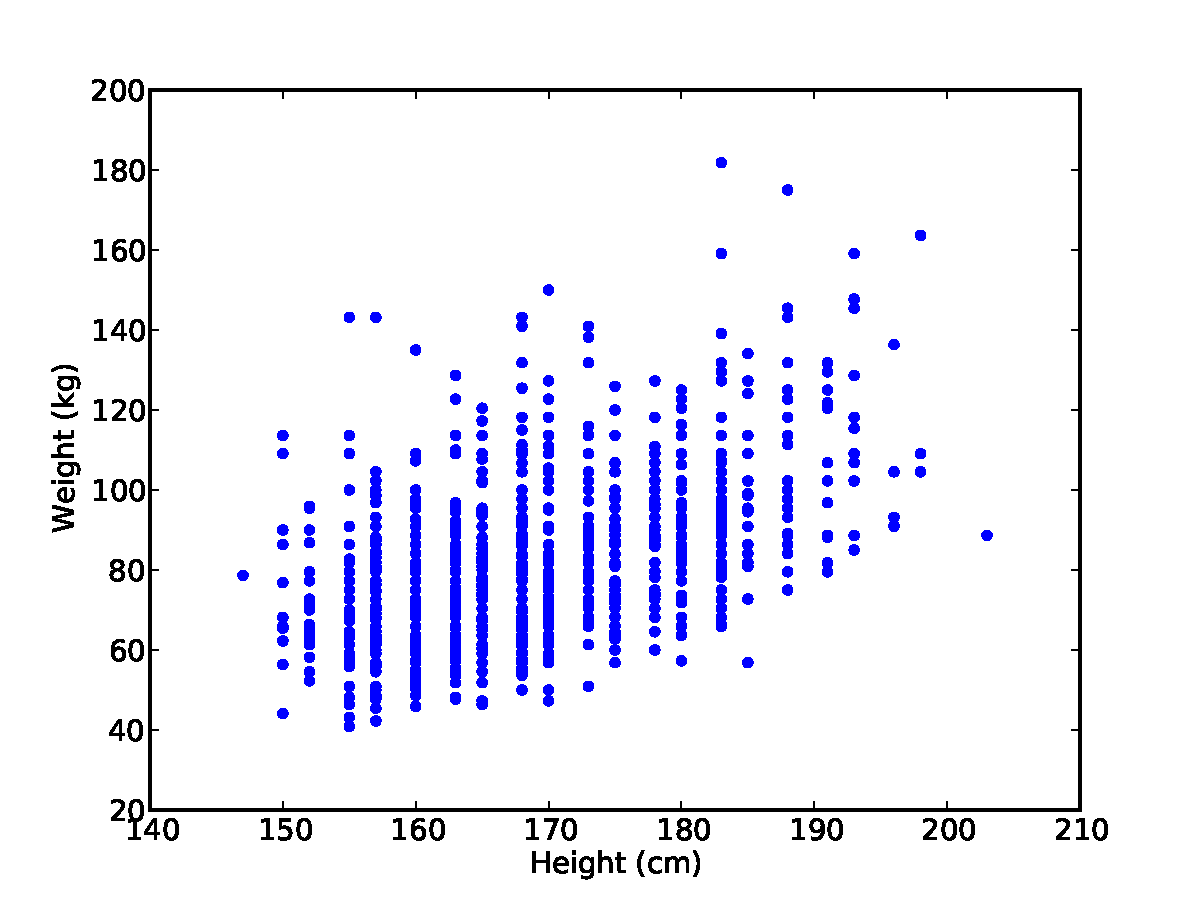
\includegraphics[height=3.0in]{figs/scatter1.pdf}}
\caption{Scatter plots of weight versus height for the respondents
in the BRFSS, unjittered (left), jittered (right).}
\label{scatter1}
\end{figure}

하지만, 상기 그림이 데이터를 가장 잘 표현하는 것은 아니다.
이유는 데이터가 열에 떼지어 몰려있다. 문제는 
신장이 가장 가까운 인치(inch) 단위로 반올림되고, 센티미터로 변환하고 나서,
다시 반올림했다. 변환 과정에서 정보가 유실되었다.

\index{신장 (height)} 
\index{체중 (weight)} 
\index{지터 (jitter)}

유실된 정보를 다시 되돌릴 수는 없지만, 데이터를 {\bf 지터링(jittering)}\footnote{jittering, 지터로 번역을 했는데 통계 사전에는 등록이 되어있지 않고 일반 사전에는 ``조금씩 움직이다''라고 나와있다.}해서 
산점도에 효과를 최소화할 수 있다. 반올림 효과를 되돌리도록 확률 잡음(random noise)를 추가한다는 의미다.
측정값이 가장 근사한 인치(inch) 정보로 반올림되어 있어서, 0.5 인치 즉, 1.3 센티미터까지 차이가 생길 수도 있다. 마찬가지로, 체중은 0.5 kg까지 차이가 생길 수 있다. 

\index{균등 분포 (uniform distribution)}
\index{분포 (distribution)!균등 (uniform)}
\index{잡음 (noise)}

%
\begin{verbatim}
    heights = thinkstats2.Jitter(heights, 1.3)
    weights = thinkstats2.Jitter(weights, 0.5)
\end{verbatim}

{\tt Jitter} 함수를 구현한 것이 다음에 있다.

\begin{verbatim}
def Jitter(values, jitter=0.5):
    n = len(values)
    return np.random.uniform(-jitter, +jitter, n) + values
\end{verbatim}

값은 임의 시퀀스가 될 수 있다; 결과는 넘파이(NumPy) 배열이다.
\index{넘파이 (NumPy)}

그림~\ref{scatter1} (오른편)에 결과가 있다.
지터링(jittering)을 통해서 반올림으로 인한 시각적 효과를 줄이고,
관계 형태를 좀더 명확히 한다. 하지만, 일반적으로 시각화 목적으로만
데이터를 지터링해야 하고, 분석을 위해서 지터링된 데이터 사용은 피해야 한다.

지터링 조차도 데이터를 표현하는 가장 최선의 방법이 되지는 못한다.
중복되는 점이 많아서 그림에서 조밀한 부분에 있는 데이터를 숨기고,
균형이 맞지 않게 특이점을 강조한다. 이와 같은 효과를 {\bf 포화 (saturation)}라고 부른다.
\index{특이점 (outlier)}
\index{포화 (saturation)}

\begin{figure}
% scatter.py
\centerline{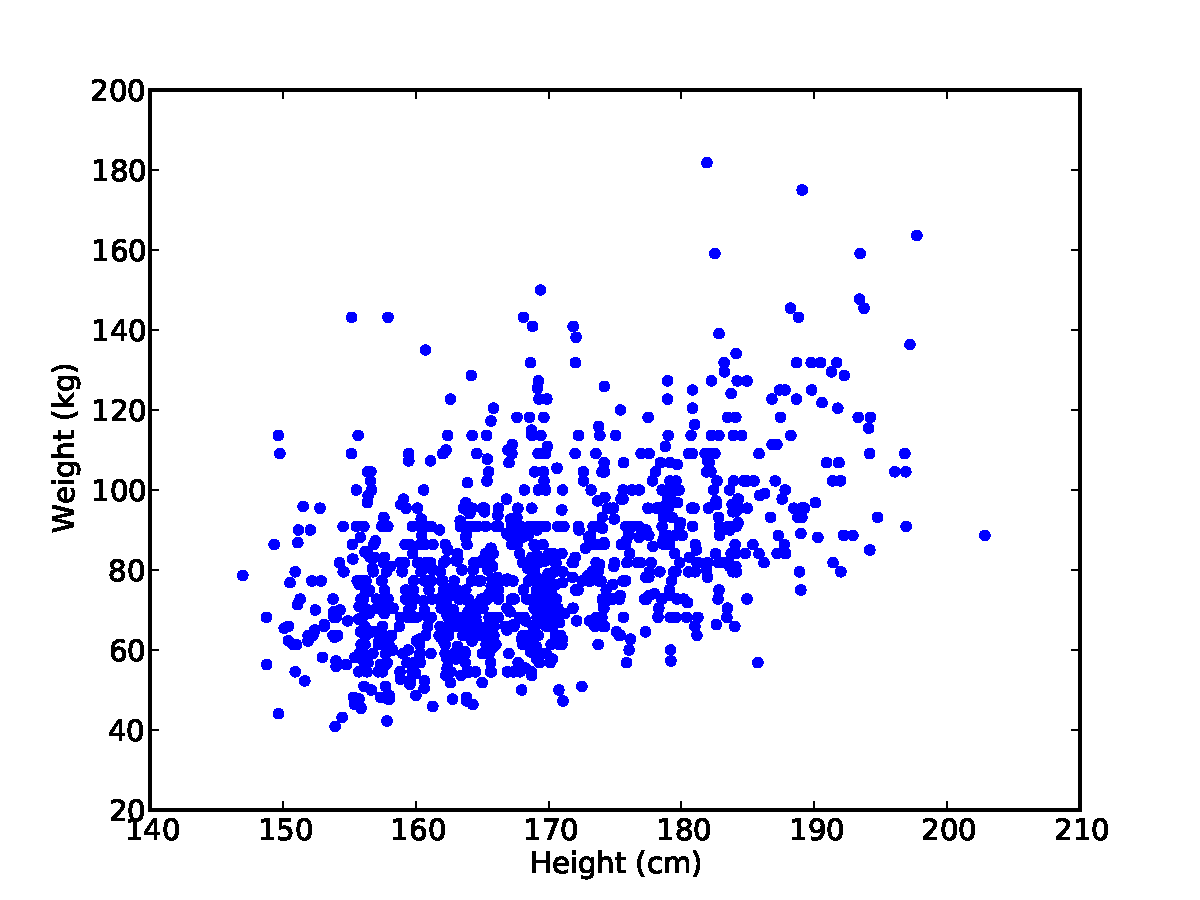
\includegraphics[height=3.0in]{figs/scatter2.pdf}}
\caption{Scatter plot with jittering and transparency (left),
hexbin plot (right).}
\label{scatter2}
\end{figure}

이런 문제를 {\tt alpha} 모수로 해결할 수 있는데, 수행하는 역할은 점들을 부분적으로 투명하게 한다.

%
\begin{verbatim}
    thinkplot.Scatter(heights, weights, alpha=0.2)
\end{verbatim}
%

그림~\ref{scatter2} (왼편)에 결과가 있다.
겹쳐지는 데이터 점들이 더 어두워 보여서 색이 짙음이 밀도와 비례하여 균형을 맞춘다. 이 버젼으로 그린 플롯을 살펴보면, 앞에서 명확하지 않은 두가지 자세한 사항을 볼 수 있다; 90 kg 즉, 200 파운드 근처에 수평선과 몇군데 신장에서 수직 군집이 보인다. 데이터가 파운드 단위로 자기 응답에 기반하기 때문에, 가장 그럴듯한 설명은 응답자가 반올림한 값으로 보고를 한 것이다.

\index{thinkplot}
\index{alpha}
\index{투영성 (transparency)}

투명성을 사용해서 중간정도 크기 데이터셋를 처리했다.
하지만, 그림은 단지 BRFSS 자료 414 509 중에서 첫 5000 레코드만 보여준다.

\index{육각함 플롯 (hexbin plot)}
\index{플롯 (plot)!육각함 (hexbin)}

더 커다란 데이터셋을 처리하기 위한,
또 다른 선택지가 육각함 플롯 (hexbin plot)이 된다.
그래프를 육각형 통(hexagonal bin)으로 나누고 각 통을 얼마나 많은 데이터가 들어있는지에 따라 색을 칠한다. {\tt thinkplot}에 {\tt HexBin}메쏘드가 있다.
%
\begin{verbatim}
    thinkplot.HexBin(heights, weights)
\end{verbatim}
%

그림~\ref{scatter2} (오른편)에 결과가 있다.
육각함(hexbin)의 장점은 관계 형태도 보여준다는 것이고,
큰 데이터셋에 대해서도 시간과 파일 크기에 둘 관점에서 효율적이다.
단점은 특이점이 보이지 않는다는 것이다.
 
\index{thinkplot}
\index{특이점 (outlier)}

이 사례를 통해서 강조하고자 하는 것은 오해를 불러 일으키는 산출물 없이 관계를 명확하게 보여주는 산점도를 플롯으로 그리는 것이 쉬운 것은 아니라는 점이다.

\index{산출물 (artifact)}


\section{Characterizing relationships}
\label{characterizing}

Scatter plots provide a general impression of the relationship between
variables, but there are other visualizations that provide more
insight into the nature of the relationship.  One option is to bin one
variable and plot percentiles of the other.
\index{binning}

NumPy and pandas provide functions for binning data:
\index{NumPy}
\index{pandas}

\begin{verbatim}
    df = df.dropna(subset=['htm3', 'wtkg2'])
    bins = np.arange(135, 210, 5)
    indices = np.digitize(df.htm3, bins)
    groups = df.groupby(indices)
\end{verbatim}

{\tt dropna} drops rows with {\tt nan} in any of the listed columns.
{\tt arange} makes a NumPy array of bins from 135 to, but not including,
210, in increments of 5.
\index{dropna}
\index{digitize}
\index{NaN}

{\tt digitize} computes the index of the bin that contains each value
in {\tt df.htm3}.  The result is a NumPy array of integer indices.
Values that fall below the lowest bin are mapped to index 0.  Values
above the highest bin are mapped to {\tt len(bins)}.

\begin{figure}
% scatter.py
\centerline{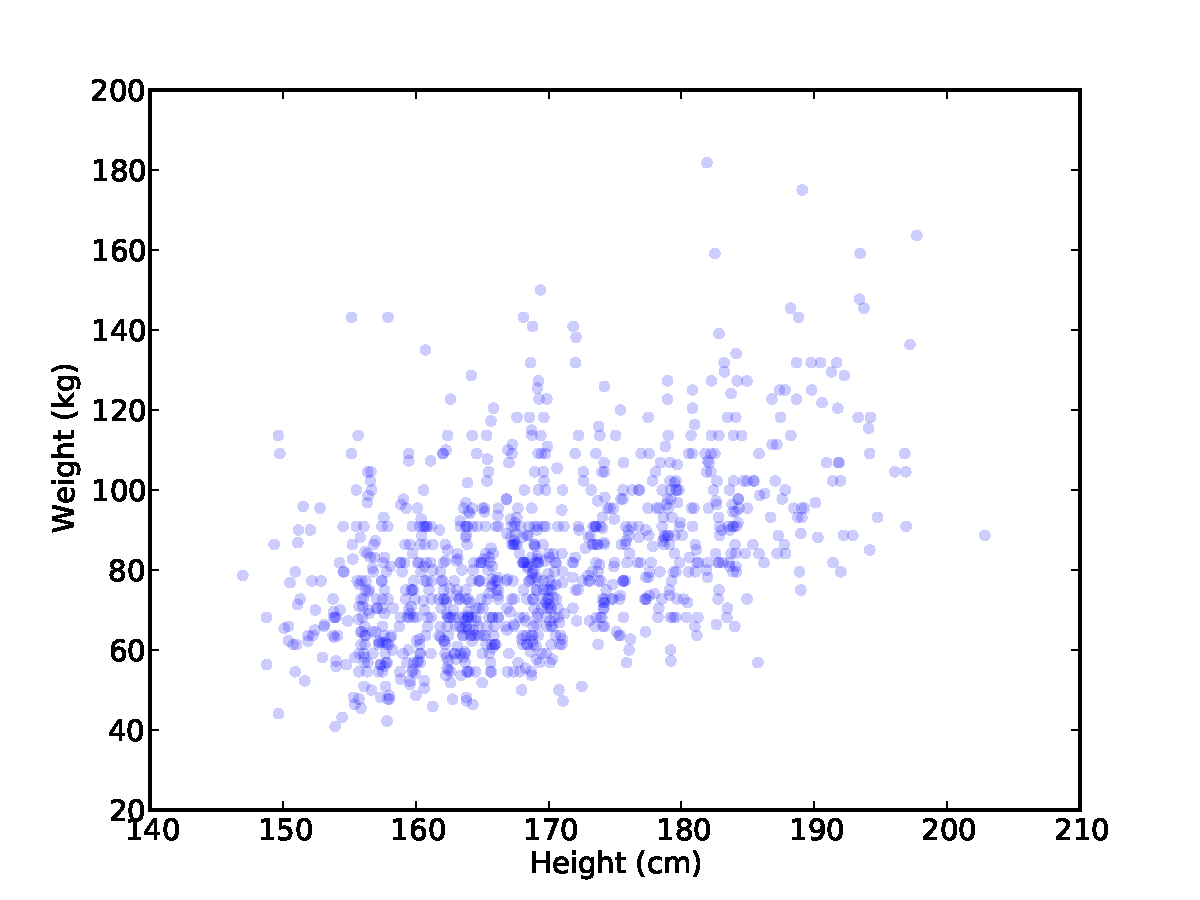
\includegraphics[height=2.5in]{figs/scatter3.pdf}}
\caption{Percentiles of weight for a range of height bins.}
\label{scatter3}
\end{figure}

{\tt groupby} is a DataFrame method that returns a GroupBy object;
used in a {\tt for} loop, {\tt groups} iterates the names of the groups
and the DataFrames that represent them.  So, for example, we can
print the number of rows in each group like this:
\index{DataFrame}
\index{groupby}

\begin{verbatim}
for i, group in groups:
    print(i, len(group))
\end{verbatim}

Now for each group we can compute the mean height and the CDF
of weight:
\index{Cdf}

\begin{verbatim}
    heights = [group.htm3.mean() for i, group in groups]
    cdfs = [thinkstats2.Cdf(group.wtkg2) for i, group in groups]
\end{verbatim}

Finally, we can
plot percentiles of weight versus height:
\index{percentile}

\begin{verbatim}
    for percent in [75, 50, 25]:
        weights = [cdf.Percentile(percent) for cdf in cdfs]
        label = '%dth' % percent
        thinkplot.Plot(heights, weights, label=label)
\end{verbatim}

Figure~\ref{scatter3} shows the result.  Between 140 and 200 cm
the relationship between these variables is roughly linear.  This range
includes more than 99\% of the data, so we don't have to worry
too much about the extremes.
\index{thinkplot}


\section{Correlation}

A {\bf correlation} is a statistic intended to quantify the strength
of the relationship between two variables.
\index{correlation}

A challenge in measuring correlation is that the variables we want to
compare are often not expressed in the same units.  And even if they
are in the same units, they come from different distributions.
\index{units}

There are two common solutions to these problems:

\begin{enumerate}

\item Transform each value to a {\bf standard scores}, which is the
number of standard deviations from the mean.  
This transform leads to
the ``Pearson product-moment correlation coefficient.''
\index{standard score}
\index{standard deviation}
\index{Pearson coefficient of correlation}

\item Transform each value to its {\bf rank}, which is its index in
the sorted list of values.  This transform
leads to the ``Spearman rank correlation coefficient.''
\index{rank}
\index{percentile rank}
\index{Spearman coefficient of correlation}

\end{enumerate}

If $X$ is a series of $n$ values, $x_i$, we can convert to standard
scores by subtracting the mean and dividing by the standard deviation:
$z_i = (x_i - \mu) / \sigma$.
\index{mean}
\index{standard deviation}

The numerator is a deviation: the distance from the mean.  Dividing by
$\sigma$ {\bf standardizes} the deviation, so the values of $Z$ are
dimensionless (no units) and their distribution has mean 0 and
variance 1.
\index{standardize}
\index{deviation}
\index{normal distribution}
\index{distribution!normal}
\index{Gaussian distribution}
\index{distribution!Gaussian}

If $X$ is normally distributed, so is $Z$.  But if $X$ is skewed or has
outliers, so does $Z$; in those cases, it is more robust to use
percentile ranks.  If we compute a new variable, $R$, so that $r_i$ is
the rank of $x_i$, the distribution of $R$ is uniform
from 1 to $n$, regardless of the distribution of $X$.
\index{uniform distribution} \index{distribution!uniform}
\index{robust}
\index{skewness}
\index{outlier}


\section{Covariance}
\index{covariance}
\index{deviation}

{\bf Covariance} is a measure of the tendency of two variables
to vary together.  If we have two series, $X$ and $Y$, their
deviations from the mean are
%
\[ dx_i = x_i - \xbar \]
\[ dy_i = y_i - \ybar \]
%
where $\xbar$ is the sample mean of $X$ and $\ybar$ is the sample mean
of $Y$.  If $X$ and $Y$ vary together, their deviations tend to have
the same sign.

If we multiply them together, the product is positive when the
deviations have the same sign and negative when they have the opposite
sign.  So adding up the products gives a measure of the tendency to
vary together.

Covariance is the mean of these products:
%
\[ Cov(X,Y) = \frac{1}{n} \sum dx_i~dy_i \]
%
where $n$ is the length of the two series (they have to be the same
length).

If you have studied linear algebra, you might recognize that
{\tt Cov} is the dot product of the deviations, divided
by their length.  So the covariance is maximized if the two vectors
are identical, 0 if they are orthogonal, and negative if they
point in opposite directions.  {\tt thinkstats2} uses {\tt np.dot} to
implement {\tt Cov} efficiently:
\index{linear algebra}
\index{dot product}
\index{orthogonal vector}

\begin{verbatim}
def Cov(xs, ys, meanx=None, meany=None):
    xs = np.asarray(xs)
    ys = np.asarray(ys)

    if meanx is None:
        meanx = np.mean(xs)
    if meany is None:
        meany = np.mean(ys)

    cov = np.dot(xs-meanx, ys-meany) / len(xs)
    return cov
\end{verbatim}

By default {\tt Cov} computes deviations from the sample means,
or you can provide known means.  If {\tt xs} and {\tt ys} are
Python sequences, {\tt np.asarray} converts them to NumPy arrays.
If they are already NumPy arrays, {\tt np.asarray} does nothing.
\index{NumPy}

This implementation of covariance is meant to be simple for purposes
of explanation.  NumPy and pandas also provide implementations of
covariance, but both of them apply a correction for small sample sizes
that we have not covered yet, and {\tt np.cov} returns a covariance
matrix, which is more than we need for now.
\index{pandas}


\section{Pearson's correlation}
\index{correlation}
\index{standard score}

Covariance is useful in some computations, but it is seldom reported
as a summary statistic because it is hard to interpret.  Among other
problems, its units are the product of the units of $X$ and $Y$.  For
example, the covariance of weight and height in the BRFSS dataset is
113 kilogram-centimeters, whatever that means.
\index{deviation}
\index{units}

One solution to this problem is to divide the deviations by the standard
deviation, which yields standard scores, and compute the product of
standard scores:
%
\[ p_i = \frac{(x_i - \xbar)}{S_X} \frac{(y_i - \ybar)}{S_Y} \]
%
Where $S_X$ and $S_Y$ are the standard deviations of $X$ and $Y$.
The mean of these products is \index{standard deviation}
%
\[ \rho = \frac{1}{n} \sum p_i \]
%
Or we can rewrite $\rho$ by factoring out $S_X$ and
$S_Y$:
%
\[ \rho = \frac{Cov(X,Y)}{S_X S_Y} \]
%
This value is called {\bf Pearson's correlation} after Karl Pearson,
an influential early statistician.  It is easy to compute and easy to
interpret.  Because standard scores are dimensionless, so is $\rho$.
\index{Pearson, Karl}
\index{Pearson coefficient of correlation}

Here is the implementation in {\tt thinkstats2}:

\begin{verbatim}
def Corr(xs, ys):
    xs = np.asarray(xs)
    ys = np.asarray(ys)

    meanx, varx = MeanVar(xs)
    meany, vary = MeanVar(ys)

    corr = Cov(xs, ys, meanx, meany) / math.sqrt(varx * vary)
    return corr
\end{verbatim}

{\tt MeanVar} computes mean and variance slightly more efficiently
than separate calls to {\tt np.mean} and {\tt np.var}.
\index{MeanVar}

Pearson's correlation is always between -1 and +1 (including both).
If $\rho$ is positive, we say that the correlation is positive,
which means that when one variable is high, the other tends to be
high.  If $\rho$ is negative, the correlation is negative, so
when one variable is high, the other is low.

The magnitude of $\rho$ indicates the strength of the correlation.  If
$\rho$ is 1 or -1, the variables are perfectly correlated, which means
that if you know one, you can make a perfect prediction about the
other.  \index{prediction}

Most correlation in the real world is not perfect, but it is still
useful.  The correlation of height and weight is 0.51, which is a
strong correlation compared to similar human-related variables.


\section{Nonlinear relationships}

If Pearson's correlation is near 0, it is tempting to conclude
that there is no relationship between the variables, but that
conclusion is not valid.  Pearson's correlation only measures {\em
  linear} relationships.  If there's a nonlinear relationship, $\rho$
understates its strength.  \index{linear relationship}
\index{nonlinear}
\index{Pearson coefficient of correlation}

\begin{figure}
\centerline{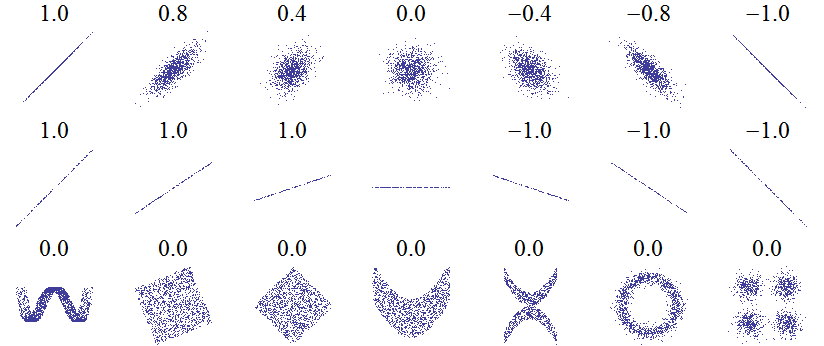
\includegraphics[height=2.5in]{figs/Correlation_examples.png}}
\caption{Examples of datasets with a range of correlations.}
\label{corr_examples}
\end{figure}

Figure~\ref{corr_examples} is from
\url{http://wikipedia.org/wiki/Correlation_and_dependence}.  It shows
scatter plots and correlation coefficients for several
carefully constructed datasets.
\index{scatter plot}
\index{plot!scatter}

The top row shows linear relationships with a range of correlations;
you can use this row to get a sense of what different values of
$\rho$ look like.  The second row shows perfect correlations with a
range of slopes, which demonstrates that correlation is unrelated to
slope (we'll talk about estimating slope soon).  The third row shows
variables that are clearly related, but because the relationship is
nonlinear, the correlation coefficient is 0.
\index{nonlinear}

The moral of this story is that you should always look at a scatter
plot of your data before blindly computing a correlation coefficient.
\index{correlation}


\section{Spearman's rank correlation}

Pearson's correlation works well if the relationship between variables
is linear and if the variables are roughly normal.  But it is not
robust in the presence of outliers.
\index{Pearson coefficient of correlation}
\index{Spearman coefficient of correlation}
\index{normal distribution}
\index{distribution!normal}
\index{Gaussian distribution}
\index{distribution!Gaussian}
\index{robust}
Spearman's rank correlation is an alternative that mitigates the
effect of outliers and skewed distributions.  To compute Spearman's
correlation, we have to compute the {\bf rank} of each value, which is its
index in the sorted sample.  For example, in the sample {\tt [1, 2, 5, 7]}
the rank of the value 5 is 3, because it appears third in the sorted
list.  Then we compute Pearson's correlation for the ranks.
\index{skewness}
\index{outlier}
\index{rank}

{\tt thinkstats2} provides a function that computes Spearman's rank
correlation:

\begin{verbatim}
def SpearmanCorr(xs, ys):
    xranks = pandas.Series(xs).rank()
    yranks = pandas.Series(ys).rank()
    return Corr(xranks, yranks)
\end{verbatim}

I convert the arguments to pandas Series objects so I can use
{\tt rank}, which computes the rank for each value and returns
a Series.  Then I use {\tt Corr} to compute the correlation
of the ranks.
\index{pandas}
\index{Series}

I could also use {\tt Series.corr} directly and specify
Spearman's method:

\begin{verbatim}
def SpearmanCorr(xs, ys):
    xs = pandas.Series(xs)
    ys = pandas.Series(ys)
    return xs.corr(ys, method='spearman')
\end{verbatim}

The Spearman rank correlation for the BRFSS data is 0.54, a little
higher than the Pearson correlation, 0.51.  There are several possible
reasons for the difference, including:
\index{rank correlation}
\index{BRFSS}

\begin{itemize}

\item If the relationship is
nonlinear, Pearson's correlation tends to underestimate the strength
of the relationship, and 
\index{nonlinear}

\item Pearson's correlation can be affected (in either direction)
if one of the distributions is skewed or contains outliers.  Spearman's
rank correlation is more robust.
\index{skewness}
\index{outlier}
\index{robust}

\end{itemize}

In the BRFSS example, we know that the distribution of weights is
roughly lognormal; under a log transform it approximates a normal
distribution, so it has no skew.
So another way to eliminate the effect of skewness is to
compute Pearson's
correlation with log-weight and height:
\index{lognormal distribution}
\index{distribution!lognormal}

\begin{verbatim}
    thinkstats2.Corr(df.htm3, np.log(df.wtkg2)))
\end{verbatim}

The result is 0.53, close to the rank correlation, 0.54.  So that
suggests that skewness in the distribution of weight explains most of
the difference between Pearson's and Spearman's correlation.
\index{skewness}
\index{Spearman coefficient of correlation}
\index{Pearson coefficient of correlation}


\section{Correlation and causation}
\index{correlation}
\index{causation}

If variables A and B are correlated, there are three possible
explanations: A causes B, or B causes A, or some other set of factors
causes both A and B.  These explanations are called ``causal
relationships''.
\index{causal relationship}

Correlation alone does not distinguish between these explanations,
so it does not tell you which ones are true.
This rule is often summarized with the phrase ``Correlation
does not imply causation,'' which is so pithy it has its own
Wikipedia page: \url{http://wikipedia.org/wiki/Correlation_does_not_imply_causation}.

So what can you do to provide evidence of causation?

\begin{enumerate}

\item Use time.  If A comes before B, then A can cause B but not the
  other way around (at least according to our common understanding of
  causation).  The order of events can help us infer the direction
  of causation, but it does not preclude the possibility that something
  else causes both A and B.

\item Use randomness.  If you divide a large sample into two
  groups at random and compute the means of almost any variable, you
  expect the difference to be small.
  If the groups are nearly identical in all variables but one, you
  can eliminate spurious relationships.
  \index{spurious relationship}

  This works even if you don't know what the relevant variables
  are, but it works even better if you do, because you can check that
  the groups are identical.

\end{enumerate}

These ideas are the motivation for the {\bf randomized controlled
trial}, in which subjects are assigned randomly to two (or more)
groups: a {\bf treatment group} that receives some kind of intervention,
like a new medicine, and a {\bf control group} that receives
no intervention, or another treatment whose effects are known.
\index{randomized controlled trial}
\index{controlled trial}
\index{treatment group}
\index{control group}
\index{medicine}

A randomized controlled trial is the most reliable way to demonstrate
a causal relationship, and the foundation of science-based medicine
(see \url{http://wikipedia.org/wiki/Randomized_controlled_trial}).

Unfortunately, controlled trials are only possible in the laboratory
sciences, medicine, and a few other disciplines.  In the social sciences,
controlled experiments are rare, usually because they are impossible
or unethical.
\index{ethics}

An alternative is to look for a {\bf natural experiment}, where
different ``treatments'' are applied to groups that are otherwise
similar.  One danger of natural experiments is that the groups might
differ in ways that are not apparent.  You can read more about this
topic at \url{http://wikipedia.org/wiki/Natural_experiment}.
\index{natural experiment}

In some cases it is possible to infer causal relationships using {\bf
  regression analysis}, which is the topic of Chapter~\ref{regression}.
\index{regression analysis}


\section{Exercises}

A solution to this exercise is in \verb"chap07soln.py".

\begin{exercise}
Using data from the NSFG, make a scatter plot of birth weight
versus mother's age.  Plot percentiles of birth weight
versus mother's age.  Compute Pearson's and Spearman's correlations.
How would you characterize the relationship
between these variables?
\index{birth weight}
\index{weight!birth}
\index{Pearson coefficient of correlation}
\index{Spearman coefficient of correlation}
\end{exercise}


\section{Glossary}

\begin{itemize}

\item scatter plot: A visualization of the relationship between
two variables, showing one point for each row of data.
\index{scatter plot}

\item jitter: Random noise added to data for purposes of
visualization.
\index{jitter}

\item saturation: Loss of information when multiple points are
plotted on top of each other. 
\index{saturation}

\item correlation: A statistic that measures the strength of the
relationship between two variables.
\index{correlation}

\item standardize: To transform a set of values so that their mean is 0 and
their variance is 1.
\index{standardize}

\item standard score: A value that has been standardized so that it is
  expressed in standard deviations from the mean.
  \index{standard score}
\index{standard deviation}

\item covariance: A measure of the tendency of two variables
to vary together.
\index{covariance}

\item rank: The index where an element appears in a sorted list.
\index{rank}

\item randomized controlled trial: An experimental design in which subjects
are divided into groups at random, and different groups are given different
treatments.
\index{randomized controlled trial}

\item treatment group: A group in a controlled trial that receives
some kind of intervention.
\index{treatment group}

\item control group: A group in a controlled trial that receives no
treatment, or a treatment whose effect is known.
\index{control group}

\item natural experiment: An experimental design that takes advantage of
a natural division of subjects into groups in ways that are at least
approximately random.
\index{natural experiment}

\end{itemize}

